
\section{Architektur}
\label{Architektur}

In diesem Kapitel wird die Architektur unserer Applikation und die Schnittstellen zu den Umsystemen besprochen.
Als Anhaltspunkt wird das C4 Modell \cite{c4model} von Simon Brown verwendet.
In einem ersten Schritt wird unsere Applikation ''ÖV-Güteklassen 2018'' in den Kontext des grösseren Systems gesetzt.
Anschliessend teilen wir das System \code{TODO} in einzelne Container und den zentralen Container \code{TODO} in einzelne Komponenten auf.

\subsection{Systemkontext}
\label{Architektur:Systemkontext}

In Abbildung \ref{fig:system-context-diagram} ist gestrichelt eingerahmt das System ''ÖV-Güteklassen 2018'' zusammen mit den dazugehörigen Umsystemen dargestellt.
Die Pfeile bedeuten, dass ein System in Richtung der Pfeilspitze Anfragen an ein anderes System sendet.
Die Daten fliessen dementsprechend in die entgegengesetzte Richtung.

\begin{figure}[ht]
    \centering
    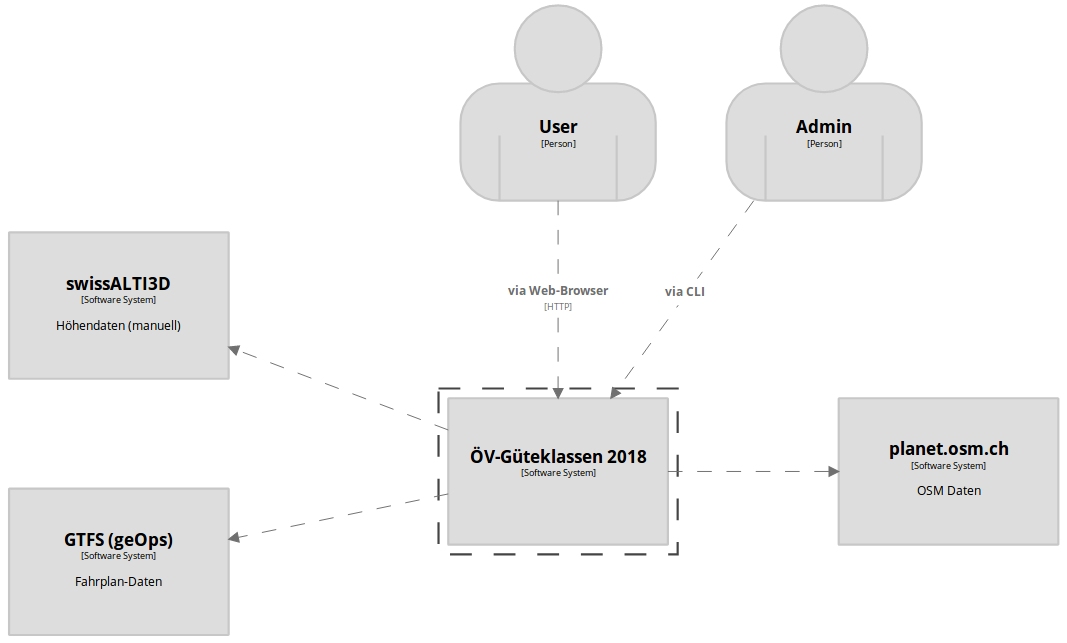
\includegraphics[width=1\linewidth]{projectdoc/img/systemcontext-diagram.png}
    \caption[Systemkontextdiagramm]{Systemkontextdiagramm ÖV-Güteklassen 2018}
    \label{fig:system-context-diagram}
\end{figure}

Im Folgenden werden die Umsysteme sowie die Beziehungen zu unserem System ''Öv-Güteklassen 2018'' genauer beschrieben.

\subsubsection{Web-App}
\label{subsystem:Web-App}

Die Web-App dient zur Darstellung der ÖV-Güteklassen in einer interaktiven Karte für den Benutzer.
Dazu erhält es die vorberechneten Daten vom System ''ÖV-Güteklassen 2018'' und visualisiert sie für die Anzeige im Webbrowser.

\subsubsection{swissALTI3D}
\label{subsystem:swissALTI3D}

Für die Höhendaten wird swissALTI3D, ein Produkt von swisstopo~\cite{swissalti3d_swisstopo}, verwendet.
Diese werden manuell bezogen, da der Datensatz mit ca. 120GB für ein Download über das Web-API zu gross ist.

Das Höhenmodell wird anschliessend in die Routing-Engine integriert, wo die Höhenunterschiede für die Kostenberechnung einer Route verwendet werden können.

\subsubsection{GTFS}
\label{subsystem:GTFS}

Die Fahrplandaten werden von der SBB regelmässig im HAFAS-Format publiziert.~\cite{sbb_hafas_spec}
Diese werden von geOps in das offene und einfacher handhabbare Format \ac{GTFS}~\cite{gtfs_spec} konvertiert und kostenfrei publiziert.~\cite{geops_fahrplandaten}

Die \ac{GTFS}-Daten im CSV-Format werden in einer relationalen Datenbank gespeichert und für die Berechnung der ÖV-Güteklassen bereit gestellt.

\subsubsection{planet.osm.ch}
\label{subsystem:planet.osm.ch}

Für die Berechnung der ÖV-Güteklassen benötigt es aktuelle Kartendaten, um die Erreichbarkeiten von Haltestellen entlang dem Strassennetz zu analysieren.
Dazu bieten sich Daten von \ac{OSM} ideal an, da sie frei verfügbar sind und kontinuierlich aktualisiert werden.

Unter planet.osm.ch werden täglich aktualisierte \ac{OSM}-Daten der ganzen Schweiz bereit gestellt.~\cite{planet_osm_ch}
Die Daten sind im \ac{PBF} und werden mit entsprechenden Tools in eine relationale Datenbank importiert, wo sie von einer Routing-Engine genutzt werden können.


\subsection{Container}
\label{Architektur:Container}

\begin{figure}[ht]
    \centering
    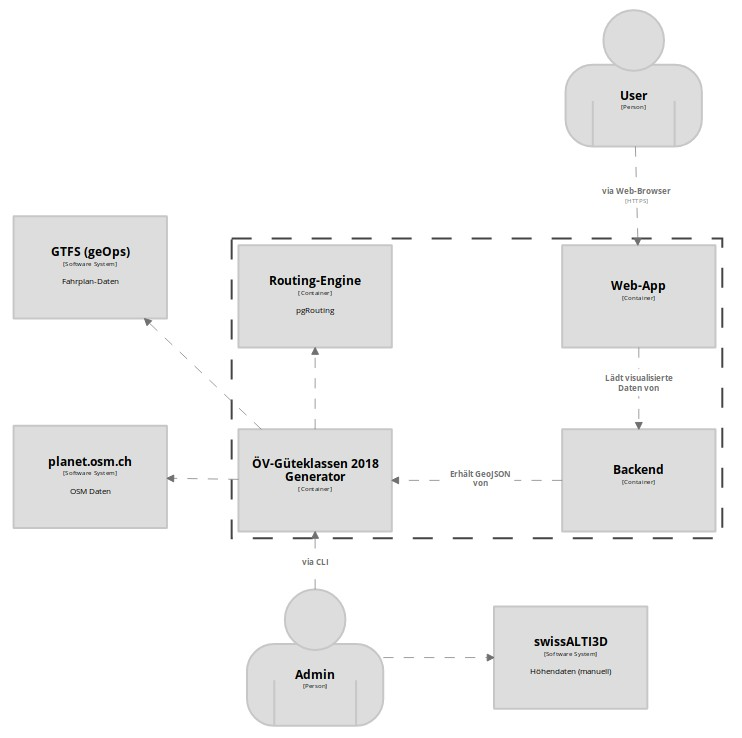
\includegraphics[width=1\linewidth]{projectdoc/img/container-diagram}
    \caption[ht]{}
    \caption[Containerdiagramm]{Containerdiagramm ÖV-Güteklassen 2018}
    \label{fig:container-diagram}
\end{figure}



\subsection{Component}
\label{Architektur:Component}

%TODO

\subsection{Code}
\label{Architektur:Code}

%TODO vlt. auf anderes Kapitel verweisen